\part{Verschlüsselung Allgemein}
\section{Sinn und Zweck der Verschlüsselung}
Die Verschlüsselung bzw. die Geheimhaltung von Informationen wurde schon lange vor Christi Geburt gebraucht. Es ist wichtig wie ich eine Information vor Unbefugten so darstellen kann, dass es für sie keinen Sinn ergibt. Mit dem geheimen Schlüssel können die Informationen jedoch gelesen werden. %Ich, oder Andere, mit einem geheimen Schlüssel können die Information jedoch lesen. 
Der Zweck der Verschlüsselung ist, dass das Lesen von Daten durch Unbefugte verunmöglicht wird. \\
Als Beispiel stellen wir uns den vertraulichen Briefverkehr zwischen zwei Freunden vor. Da sie dem Briefträger und der Schweizerischen Post vertrauen, verschlüsseln wir in der Regel die Briefe nicht. Mit einem Siegel und dem Briefumschlag würden wir bemerken, falls jemand den Brief vorzeitig geöffnet hat. Zusätzlich können wir mit einem Siegel und der Unterschrift die Authentizität des Absenders verifizieren.\\
Im Gegensatz zu dem Brief können wir uns bei einer Email nicht auf diese Sicherheiten verlassen. Eine Email wird über verschiedenste Server und Länder gesendet, bis sie über einen Weg aus mehreren Knotenpunkten beim Empfänger ankommt. Wer und ob diese Nachricht sonst noch kopiert, geöffnet oder gelesen wurde ist nicht nachvollziehbar. Daher brauchen wir eine Verschlüsselung, damit nur der gewünschte Empfänger diese Nachricht entschlüsseln und somit auch lesen kann.
%
%Im realen Leben können wir zum Beispiel unser Haus vor Dieben sichern, indem wir eine Türe mit einem stabilen Schloss einbauen. Möchte man noch weiter gehen, kann man eine Alarmanlage einbauen.\\[2ex]
%
% In der Digitalen Welt geht das nicht so einfach. Obwohl man seinen Rechner mit einem Benutzername und Passwort für unbefugte Personen schützen kann, gibt es Techniken, mit der lassen sich ganze Festplatten Bit für Bit kopieren. Hier setzt die Verschlüsselung an. Denn wenn man etwas verschlüsselt auf die Festplatte speichert, kann der unbefugte die gestohlenen Daten nicht brauchen.
%\section{Geschichte der Verschlüsselung}
\section{Klassische Kryptographie}
Die Kryptographie bezeichnet die Entwicklung von Methoden zur Verheimlichung von Nachrichten. Das Wort Kryptographie setzt sich aus dem Griechischen Wort \textit{kryptos} und \textit{graphein} zusammen, was so viel wie \textit{"verborgen schreiben"} heisst.% (Siehe Kapitel \cite{kryptographie_Grundlagen} ) \\
Die Hebräer haben 600 vor Christus das Atbash entwickelt. Dabei wurde das Alphabet umgekehrt und entsprechend verschlüsselt.
%
\begin{table}[ht]
\caption{Atbash Verschlüsselung}
\begin{center}
\begin{tabular}{|l|l|l|l|l|l|l|}
  a & b & c & d & e & f\\
  z & y & x & w & v & u\\
\end{tabular}
\end{center}
\end{table} \\
%
Das Wort GIBM wird mit Atbash zu TRYN.\\
Die Caesar-Verschlüsselung wurde nach Julius Caesar benannt und zur militärischen Korrespondenz im Römischen Reich gebraucht.\\
Dafür wurde das Alphabet um 3 Stellen nach hinten verschoben. Aus einem D wird somit ein A. Dieses Verfahren wurde im 15. Jahrhundert mit einer Chiffrierscheibe verbessert und ist bis heute noch als Caesar Verschlüsselung bekannt. Die Verschiebung um 13 Stellen wird auch als rot13 bezeichnet, da unser Alphabet aus 26 Zeichen besteht, ist die Verschlüsselung und Entschlüsselung bei rot13 die selbe. (Siehe Kapitel 1.2 \cite{kryptographie_Grundlagen} ) \\
%
\begin{table}[ht]
\caption{Caesar Verschlüsselung}
\begin{center}
\begin{tabular}{|l|l|l|l|l|l|l|}
  a & b & c & d & e & f\\
  x & y & z & a & b & c\\
\end{tabular}
\end{center}
\end{table}
%
Aus GIBM wird mit der Ceasar Verschlüsselung DFYJ \\
%
Diese Verfahren können einfach geknackt werden. Da bestimmte Buchstaben in einer Sprache öfter vorkommen, kann durch Textanalyse die Verschiebung herausgefunden werden. Ebenfalls wird der Grundsatz verletzt, dass die Sicherheit nicht von der Geheimhaltung des Algorithmus abhängen darf. (Vergleiche Kerckhoff's Prinzip Kapitel \ref{sec:Probleme_der_frueheren_Verschluesselungen} )
%
%%%%%%%%%%%%%%%%%%%%%%%%%%%%%%%%%%%%%%%%%%%%%%%%%%%%%
% Enigma und 2ter Weltkrieg
%%%%%%%%%%%%%%%%%%%%%%%%%%%%%%%%%%%%%%%%%%%%%%%%%%%%%
%
\subsection{Kryptographie im zweiten Weltkrieg}
Für dieses Kapitel wurde die Dissertation \textit{Chiffriermaschinen und Entzifferungsgeräte
im Zweiten Weltkrieg: Technikgeschichte und informatikhistorische Aspekte} \cite{enigma} verwendet, da diese Arbeit alle Bereiche der Enigma abdeckt. \\
Im zweiten Weltkrieg nutzte die Deutsche Wehrmacht die Enigma zur Verschlüsselung ihres Funkverkehrs. Die Enigma ist einer Schreibmaschine ähnlich und besteht aus einer Tastatur, einem Walzensatz und einer Anzeige über Lampen. 
%
\begin{figure}[ht]
\begin{center}
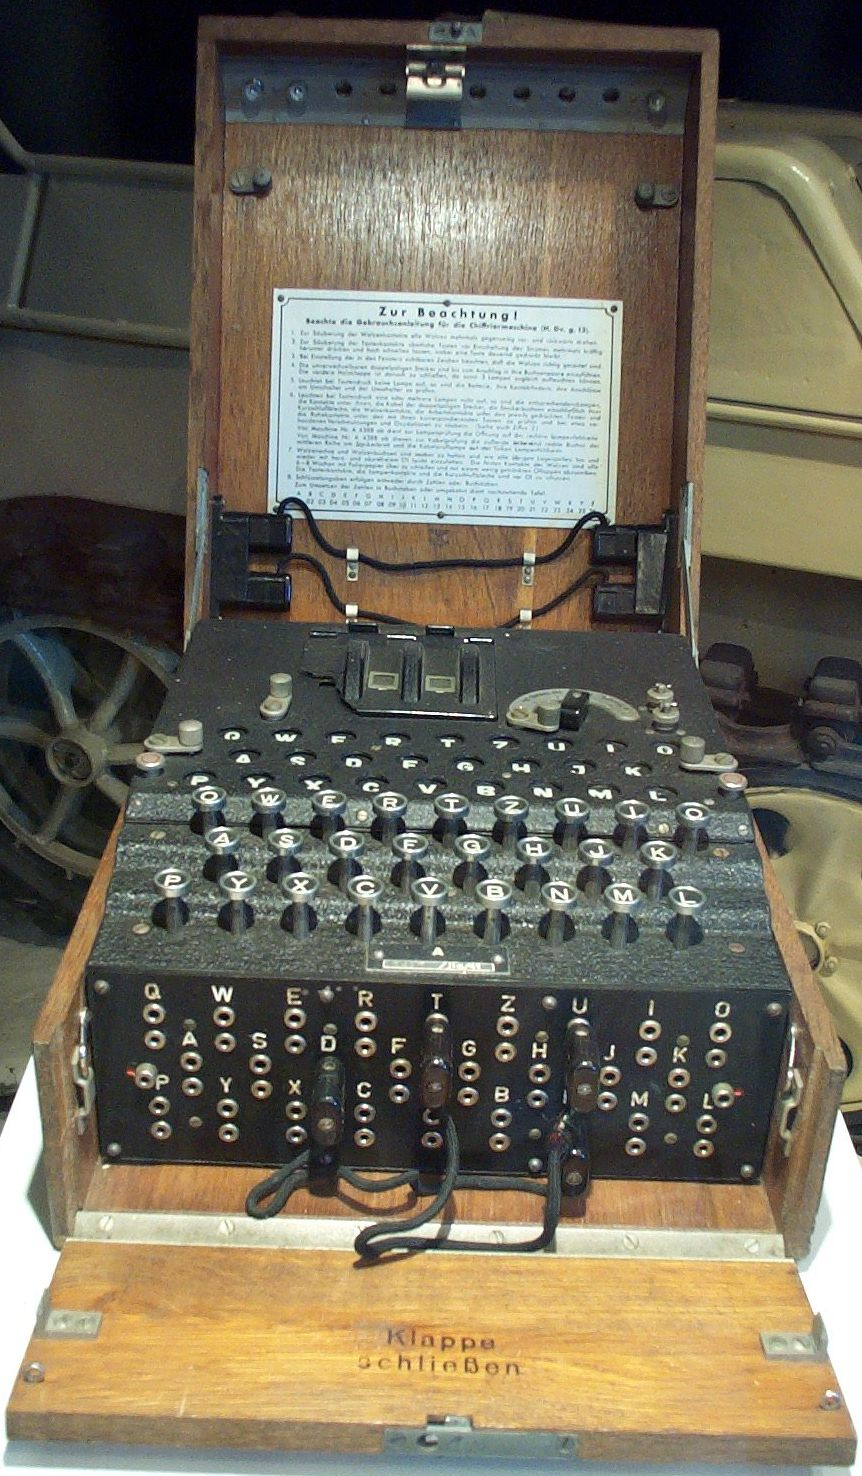
\includegraphics[height=5cm]{images/Enigma_Verkehrshaus_Luzern_cropped.jpg}
\caption[Enigma Maschine Quelle:\newline ~~~~http://upload.wikimedia.org/wikipedia/commons/d/d1/\newline Enigma\_Verkehrshaus\_Luzern\_cropped.jpg]{Enigma Maschine}
\label{fig:enigma}
\end{center}
\end{figure}
%
\subsubsection{Funktion der Enigma Maschine}
Die Walzen können sich drehen und sind mit elektrischen Kontakten miteinander verbunden. Wird eine Taste gedrückt, fliesst Strom durch den Walzensatz und es leuchtet die Lampe des verschlüsselten Buchstabens auf. Dieser Stromfluss wird in Abbildung \ref{fig:stromfluss} gezeigt. Die Walze dreht sich nach jedem Tastendruck weiter, so das der gleiche Buchstabe jeweils anders verschlüsselt wird, somit kann aus AAA z. B. DXB werden. Nach 26 Umdrehungen der ersten Walze wird die zweite Walze gedreht. \\
%
\begin{figure}[ht]
\begin{center}
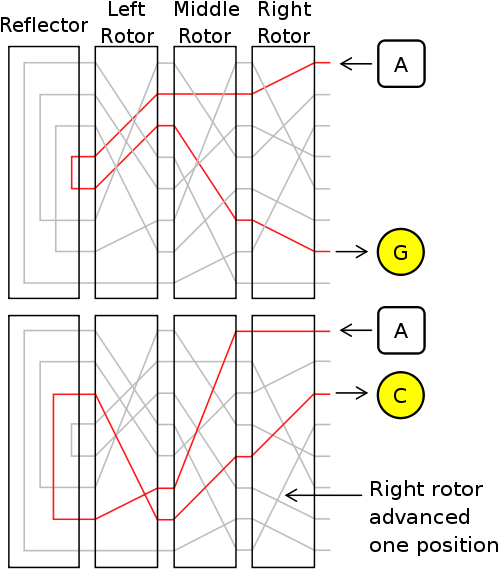
\includegraphics[width=5cm]{images/Enigma-action.png}
\caption[Enigma Stromfluss Quelle:\newline ~~~~http://upload.wikimedia.org/wikipedia/commons/6/6c/Enigma\-action.svg]{Enigma Stromfluss}
\label{fig:stromfluss}
\end{center}
\end{figure}
%
Die elektrischen Impulse durch die Walze legen nach jeder Drehung eine andere Strecke zurück. 
Über das Steckbrett konnte der verschlüsselte Buchstaben nochmals ersetzt werden. Wenn E mit J verbunden ist und nach dem verschlüsseln ein E herauskam, wird dieses mit einem J verschlüsselt. 
%
\subsubsection{Anwendung}
Die Deutsche Wehrmacht nutzte die Enigma um ihre Funksprüche zu verschlüsseln. Dazu wurden jeweils um Mitternacht die Walzen und die Steckverbindungen ausgetauscht beziehungsweise umgesteckt. Ein neuer Schlüsselsatz sah beispielsweise so aus:\\
%
%Quelle Wikipedia%
\begin{table}[ht]
\caption[Schlüsseltafel der Wehrmacht Quelle:\newline ~~~~http://de.wikipedia.org/wiki/Enigma\_\%28Maschine\%29]{Schlüsseltafel der Wehrmacht}
\begin{center}
\begin{tabular}{|l|l|l|l|l}
Tag & UKW & Walzenlage & Ringstellung &  Steckerverbindungen \\
 31  &   B   &  I   IV III   &    16 26 08   &  AD CN ET FL GI JV KZ PU QY WX \\
\end{tabular}
\end{center}
\end{table}
%
\\
Die eigentliche Verschlüsselung war relativ simpel zu bewerkstelligen. Es musste nur die entsprechende Funknachricht eingegeben werden und die Enigma erledigte die Verschlüsselung. Der Austausch der aktuellen Walzenstellung und das Morsen der Nachricht waren jedoch komplizierter.
%
Vor der eigentlichen Nachricht wurde ein Nachrichtenkopf gemorst. In diesem wurde die Länge des Textes bekannt gegeben, die Walzenstellung und die Nachrichtenart. 
Der eigentliche Text wurde in Gruppen aus 5 Buchstaben gemorst. Bei den ersten 5 Buchstaben wurde bestimmt, an wen die Nachricht geht. Dabei wurden die ersten zwei Buchstaben zufällig ausgewählt und die letzten 3 durchmischt. Nach der Alphabetischen Ordnung, konnte über eine Tabelle festgestellt werden, ob die Nachricht entschlüsselt werden darf.
Die Walzenstellung wurde verschlüsselt übertragen. Wenn im Kopf z. B. QWE EWG angegeben wurde, musste man die Walze auf die Buchstaben QWE einstellen und EWG eingeben. Was dabei verschlüsselt heraus kam, war die Anfangsstellung der Walzen, um die Nachricht zu entschlüsseln. Jetzt konnte mit der Entschlüsselung der Nachricht begonnen werden.
%
\subsubsection{Schwachstelle der Enigma}
Die Enigma benutzte ein symmetrisches Verfahren, daher war der Schlüssel für die Entschlüsselung und Verschlüsselung identisch. %TODO: Siehe Kapitel \ref{moderne Kryptographie %
Die Geheimhaltung der Walzen war wichtig, da sie einen wesentlichen Teil der Verschlüsselung ausmachen.
%Dadurch das ein Buchstabe nicht in sich selbst verschlüsselt werden kann (Strom kann nicht zurück fliessen) konnte ein wesentlicher Teil ausgeschlossen werden.
Ein Buchstabe kann nicht in sich selbst verschlüsselt werden, da der Stromfluss immer einen Anfangs- und Endpunkt benötigt. Diese Punkte können nach der Bauart der Maschine nicht gleich sein. Siehe Abbildung \ref{fig:stromfluss}
Nun konnte durch einsetzen bestimmter Wörter, welche im Text vermutet wurden, ein grosser Teil der möglichen Positionen ausgeschlossen werden. Dafür wurde z. B. OBERKOMMANDODERWEHRMACHT eingesetzt und falls an einer Position der Buchstabe in sich selbst verschlüsselt war, konnte das Wort an dieser Position nicht sein. Für die Ausnützung dieser Schwachstelle bauten die Engländer Maschinen, welche diese Arbeit vereinfachten. Die sogenannte Turing Bombe konnte nun mit den entsprechenden Walzen in 6 Stunden die Verschlüsselung knacken. 
Mit mehreren Turing Bomben wurde die Verschlüsselung in kurzer Zeit geknackt. 
%
\subsection{Probleme der früheren Verschlüsselungen}
\label{sec:Probleme_der_frueheren_Verschluesselungen}
Die Verfahren bis zum zweiten Weltkrieg konnten einfach geknackt werden. Wenn die Art der Verschlüsselung bekannt war, konnte der Schlüssel einfach ermittelt werden. 
Die Enigma revolutionierte die Kryptographie. Obwohl die Art der Verschlüsselung und sogar die Walzen bekannt waren, mussten die Engländer grosse Anstrengungen unternehmen, damit sie die Texte entschlüsseln konnten. \\[2ex]
Mit mehreren Turing Bomben wurde die Verschlüsselung in kurzer Zeit geknackt. \\[2ex]
%
Die früheren Verschlüsselungen hielten sich nicht an das Kerckhoff's Prinzip. Dieses besagt, dass die Sicherheit der Verschlüsselung nicht von der Geheimhaltung des Algorithmus abhängig gemacht werden darf. Die Sicherheit darf nur durch den Schlüssel gegeben sein. (Siehe Folie 6 \cite{kerckhoffsprinzip} )
%